\documentclass[13]{article}
\title{Digitale Bildverarbeitung}


\usepackage[a4paper, total={7in, 10.5in}]{geometry}
\usepackage{graphicx}



\newcommand*{\captionsource}[2]{%
  \caption[{#1}]{%
    #1%
    %\\\hspace{\linewidth}%
    %\textbf{Quelle:} #2%
  }%
}

\begin{document}
\section{Digitale Bildverarbeitung}
\subsection{Definition Bild}
Ein zweidimensionales Bild(2D-Bild) kann mit einer Funktion $\vec{f}(x,y)$ beschrieben werden.\\
Es existieren verschiedene Arten um 2D-Bilder darzustellen, diese unterscheiden sich in den Werten die $\vec{f}(x,y)$ zurückliefert. In dieser Arbeit behandeln wir Bilder die aus Graustufen oder aus rot-grün-blau(RGB) Anteilen besteht. Daher folgende Definition der Funktionswerte:\\\newline
\textbf{Graustufen:}(Beispiel siehe Abbildung \ref{fig:lena_gray})\\
$f(x,y) = \{a\} \;mit\;a \in M$
\begin{figure} [ht]
  \centering
  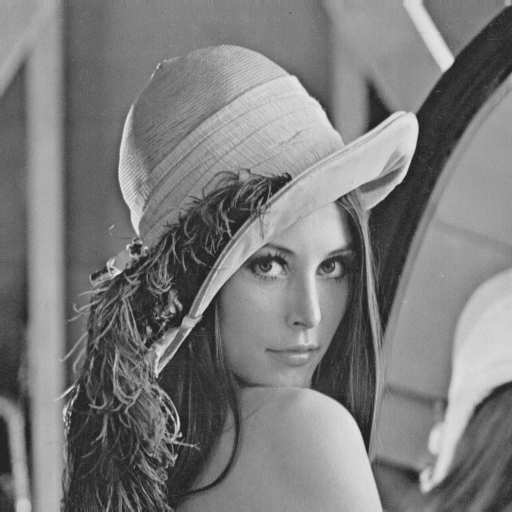
\includegraphics[height=8cm,width=8cm]{Bilder/lena_gray}
  \captionsource{Graustufen Lena, mit M = [0-512]}{https://www.cosy.sbg.ac.at/~pmeerw/Watermarking/lena.html}
  \label{fig:lena_gray}
\end{figure}\\
\\
\textbf{RGB:}(Beispiel siehe Abbildung \ref{fig:lena_rgb})\\
$f(x,y) = \{r,g,b\} \;mit\;r,g,b \in M$
\begin{figure} [ht]
  \centering
  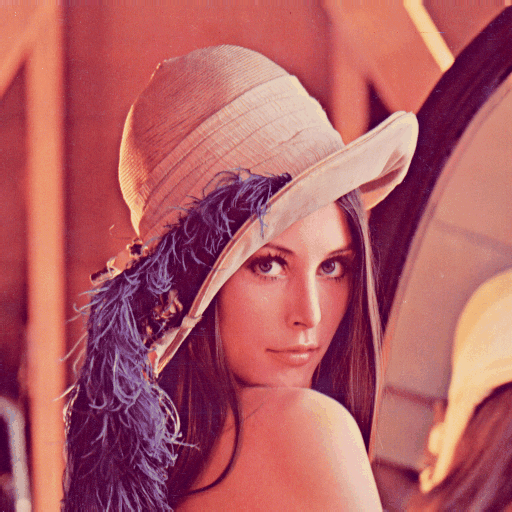
\includegraphics[height=8cm,width=8cm]{Bilder/lena_rgb}
  \captionsource{RGB Lena, mit M = [0-255]}{https://www.cosy.sbg.ac.at/~pmeerw/Watermarking/lena.html}
  \label{fig:lena_rgb}
\end{figure}
\newpage



\end{document}